\begin{wrapfigure}{r}{0.5\textwidth}
    \centering
    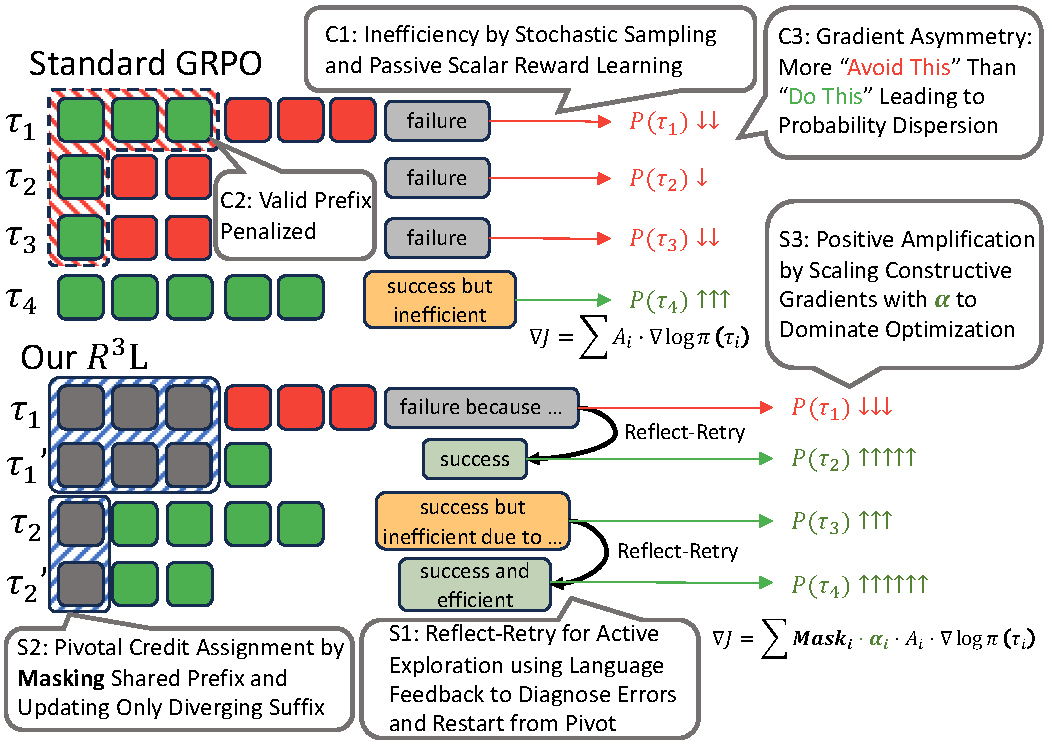
\includegraphics[width=\linewidth]{figure/src/motivation.pdf}
    \caption{Comparison between standard RL (GRPO) and R$^3$L. \textcolor{red}{Red} blocks indicate erroneous steps, \textcolor{green!50!black}{Green} blocks indicate correct steps, and \textcolor{gray}{Gray} blocks indicate masked prefix excluded from gradient updates. Standard RL suffers from (C1) inefficient stochastic sampling, (C2) valid prefix penalization, and (C3) gradient asymmetry due to failure dominance. R$^3$L addresses these via (S1) reflect-then-retry for active exploration, (S2) pivotal credit, and (S3) positive amplification. The detailed R$^3$L framework is illustrated in Figure~\ref{fig:architecture}.}
    \label{fig:motivation}
\end{wrapfigure}
